\documentclass[11pt,a4paper]{ivoa}
\input tthdefs

\usepackage{todonotes}
\usepackage{enumitem}

\usepackage{listings}
\lstloadlanguages{XML,sh}
\lstset{flexiblecolumns=true,tagstyle=\ttfamily,
showstringspaces=False}

\usepackage{multirow}

\title{Simple Cone Search}

\ivoagroup{Data Access Layer}

\author[http://www.ivoa.net/twiki/bin/view/IVOA/RayPlante]{Raymond Plante}
\author[http://www.ivoa.net/twiki/bin/view/IVOA/MarcoMolinaro]{Marco Molinaro}
\author[http://www.ivoa.net/twiki/bin/view/IVOA/MarkusDemleitner]{Markus Demleitner}
\author[http://www.ivoa.net/twiki/bin/view/IVOA/BobHanisch]{Robert Hanisch}
\author[http://www.ivoa.net/twiki/bin/view/IVOA/AlexSzalay]{Alex Szalay}
\author[http://www.ivoa.net/twiki/bin/view/IVOA/RoyWilliams]{Roy Williams}

\editor{Ray Plante, Marco Molinaro}

\previousversion[http://www.ivoa.net/Documents/REC/DAL/ConeSearch-20080222.html]{REC 1.03}
\previousversion[http://www.ivoa.net/Documents/PR/DAL/ConeSearch-20070914.html]{PR 2007-09-14}
\previousversion[http://www.ivoa.net/Documents/PR/DAL/ConeSearch-20070628.html]{PR 2007-06-28}
\previousversion[http://www.ivoa.net/Documents/PR/DAL/ConeSearch-20060908.html]{PR 2006-09-08}
       

\begin{document}
\begin{abstract}
This specification defines a simple query protocol, named Simple Cone Search (SCS or simply cone search hereafter), for retrieving records from a catalog of astronomical sources. The query describes a sky position and an angular distance, defining a cone on the sky. The response returns a list of astronomical sources from the catalog whose positions lie within the cone, formatted as a VOTable. This version aims essentially at aligning this specification with the Data Access Layer (DAL) landscape at the time of writing.
\end{abstract}


\section*{Acknowledgments}
This document was originally published as a document of the US National Virtual Observatory (NVO) \todo{check if the document or a link is still available} and then transcripted into an IVOA standards document format to became an IVOA recommendation. The changes made in this transcription and in the process of producing the first recommandation are reported in Appendix \ref{app:changes}.

The Simple Cone Search (SCS) version 1.03 document has been developed with support from the National Science Foundation's Information Technology Research Program under Cooperative Agreement AST0122449 with The Johns Hopkins University.

The SCS-1.1 revision has been developed under the ASTERICS project, supported by the European Commission Framework Programme Horizon 2020 Research and Innovation action, grant agreement n. 653477.

Work of the original authors of the Cone Search specification as well as the numerous data providers who have implemented and continue to support this protocol is kindly acknowledged.

\section*{Conformance-related definitions}

The words ``MUST'', ``SHALL'', ``SHOULD'', ``MAY'', ``RECOMMENDED'', and
``OPTIONAL'' (in upper or lower case) used in this document are to be
interpreted as described in IETF standard RFC2119 \citep{std:RFC2119}.

The \emph{Virtual Observatory (VO)} is a
general term for a collection of federated resources that can be used
to conduct astronomical research, education, and outreach.
The \href{http://www.ivoa.net}{International
Virtual Observatory Alliance (IVOA)} is a global
collaboration of separately funded projects to develop standards and
infrastructure that enable VO applications.


\section{Introduction}

This specification describes how a provider of an astronomical source catalog can publish that catalog to the Virtual Observatory in such a way that a simple cone search can be done. The data remains in the control of the data provider, served through a web server to the world, but the query profile and response profile are carefully controlled, as described below. It is intended that setting up this web service be simple enough that data providers will not have to spend too much time on it (their funding to support such services is typically small). At the same time, the service implementation and the data it provides can serve as a basis for more sophisticated tools.

This specification does not specify how cone search services are implemented, or how the data are stored or manipulated. The concern of this specification is how the data are exposed to the world through well-defined requests and responses.

This specification assumes that the data provider has already selected a catalog of astronomical sources. This catalog can be presented as a single table; it is expected that the table contains several columns.

\subsection{Role within the VO Architecture}

\begin{figure}
\centering

% Get the architecture diagram from the TCG chair
% http://wiki.ivoa.net/twiki/bin/view/IVOA/IvoaTCG
% If they give you a PDF, for now dumb it down to a png by
% convert -antialias -density 72x72 archdiag.pdf archdiag.png
% Oh -- Notes don't need this; you'd have to remove archdiag.png
% from FIGURES in the Makefile, too.

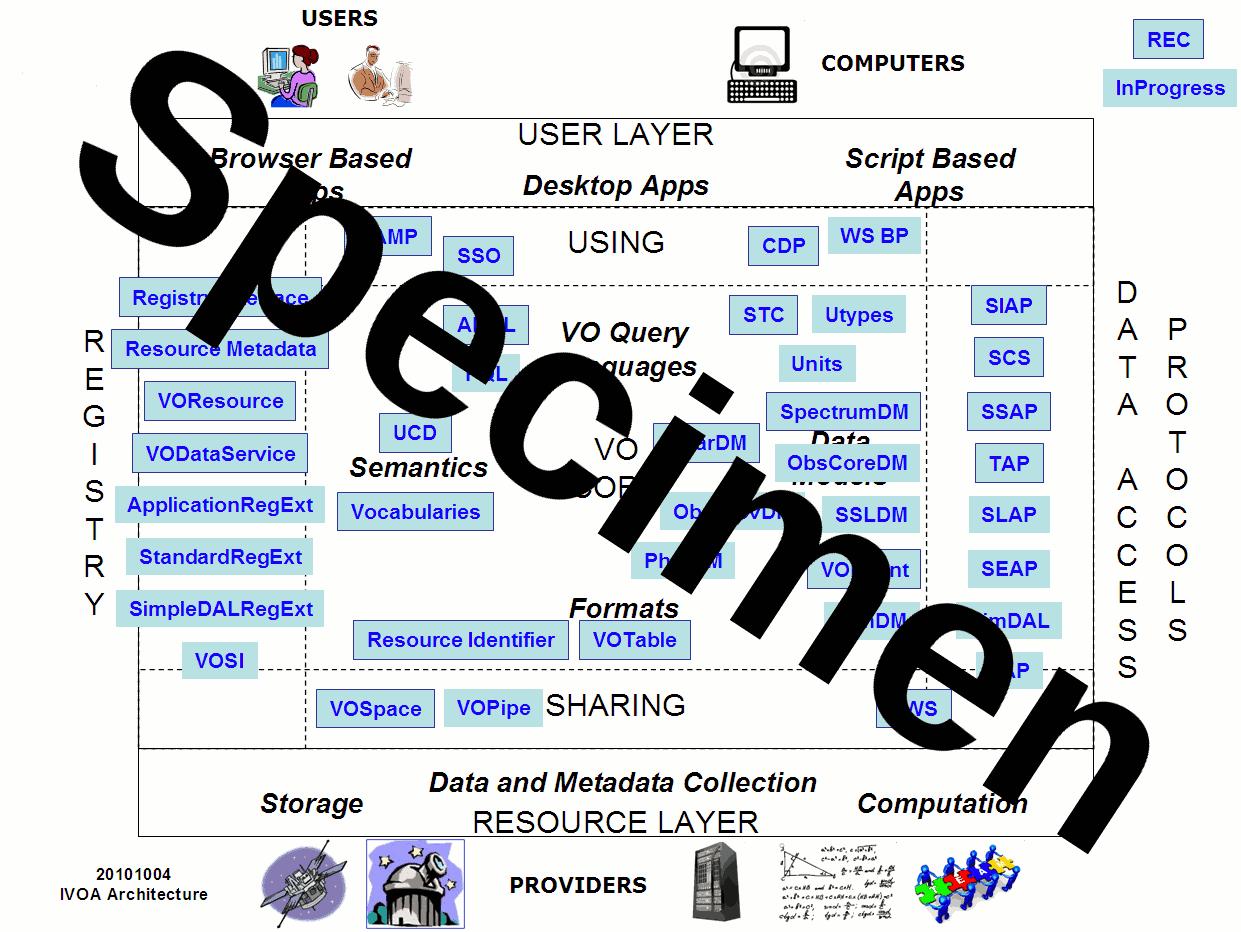
\includegraphics[width=0.9\textwidth]{archdiag.png}
\caption{Architecture diagram for SCS - TODO}
\label{fig:archdiag}
\end{figure}

Fig.~\ref{fig:archdiag} shows the role this document plays within the
IVOA architecture \citep{note:VOARCH}.

\section{Resource}
\label{sec:resif}

A SCS service for accessing catalogue resources is implemented as a synchronous resource, as compliant as possible to the DALI specification \citep{std:DALI}.

\begin{table}[th]
\begin{center}
\begin{tabular}{p{0.25\textwidth}p{0.25\textwidth}p{0.25\textwidth}}
\sptablerule
\textbf{resource type}&\textbf{resource name}&\textbf{required}\\
\sptablerule
\{query\} & service specific & yes\\
VOSI-capabilities & /capabilities & should\\
VOSI-availability & (/availability) & should\\
\sptablerule
\label{table:resources}
\end{tabular}
\caption{SCS resources tree}
\end{center}
\end{table}

It \textbf{must} have one \{query\} resource and \textbf{should} have a VOSI-capability resource and a VOSI-availability one. The VOSI-capability \textbf{must} be a sibling to the \{query\} one.

\subsection{\{query\} resource}
\label{sec:basepar}
The SCS \{query\} resource \textbf{must} meet the following requirements:
\begin{itemize}
	\item the resource \textbf{must} respond to requests submitted using an HTTP GET query string, and \textbf{should} respond to HTTP POST query actions, as described in Sec.~\ref{sec:basepar};
	\item the response, by default, \textbf{must} be a valid VOTable document, providing a table containing the sources of the catalogue whose positions are within the cone described in the query request (see Sec.~\ref{sec:response});
	\item in case of error, the response \textbf{must} follow prescriptions as described in Sec.~\ref{sec:error}.
\end{itemize}

The SCS service \texttt{\{query\}} resource is a synchronous web resource, as described by DALI, of the form
$$\hbox{\nolinkurl{http://<server>/<local_path>?} .}$$
To this base URL the query parameters, described herafter, are attached to build the query request to be submitted through HTTP.

Usage of fixed, custom query parameters, defined by the service provider to build a base URL of the form
$$\hbox{\nolinkurl{http://<server>/<local_path>?<base\_query>&}}$$
(standard behaviour of base URLs in SCS-1.03) is allowed but \textbf{deprecated} in order to bring cone searches base URLs in the common ReST DALI shape. Clients \textbf{must} anyway treat opaquely this fixed \texttt{<base\_query>} addition.

In the case of HTTP POST action, the behaviour of SCS services having the deprecated base URL format (including custom extra parameters) is not specified, because it is not defined whether the query method has to be a pure POST action or a mixed GET/POST request.

On the opposite, service having \texttt{\{query\}} base URL as mandated by this specification are highly encouraged to support HTTP POST method in order to fulfill DALI compliance.

The set of query constraints a cone search needs to understand \textbf{must} include the \textbf{RA}, \textbf{DEC}, \textbf{SR} parameters, \textbf{should} include the \textbf{MAXREC} and \textbf{RESPONSEFORMAT} ones and \textbf{may} include the \textbf{VERB} one, all of which are to be interpreted with the following stated meaning and the DALI recommendations about parameters.

\subsubsection{RA}
\textbf{RA} represents a right-ascension in the ICRS coordinate system for the position of the center of the cone to search, given in decimal degrees. It is a single valued parameter and \textbf{must} be present in the query.

\subsubsection{DEC}
\textbf{DEC} represents a declination in the ICRS coordinate system for the position of the center of the cone to search, given in decimal degrees. It is a single value parameter and \textbf{must} be present in the query.

\subsubsection{SR}
\textbf{SR} represents the radius of the cone to search, given in decimal degrees. It is a single valued parameter and \textbf{must} be present in the query. If set to zero (SR=0) it should have the same effect as setting MAXREC=0, i.e. a service metadata request as prescribed by DALI\footnote{SR=0 is kept in this version of this specification for back compatibility. It is suggested to prefer the usage of MAXREC to enable metadata discovery}.

\subsubsection{MAXREC}
As defined by DALI a cone search \textbf{should} accept the \textbf{MAXREC} parameter to let the client limit the number of records returned or require a service metadata response (see above).  Its usage is encouraged and preferred to the SR=0 solution for metadata discovery.

\subsubsection{RESPONSEFORMAT}
\label{subsubsec:responseformat}
An SCS service \textbf{must} provide responses in VOTable \citep{std:VOTABLE} format, compliant with respect to what will be detailed in Sec.~\ref{sec:response}, but \textbf{should} also support the DALI \textbf{RESPONSEFORMAT} parameter. Allowed media types for VOTable response \textbf{should} be the \texttt{application/x-votable+xml} or \texttt{text/xml} as specified by DALI but \texttt{text/xml;content=x-votable} may be considered legal for backward compatibility reasons.

\subsubsection{VERB}
The query \textbf{may} contain the optional single valued parameter, \textbf{VERB}, whose value is an integer (either 1, 2, or 3) indicating verbosity which determines how many columns are to be returned in the resulting table. If the service supports the parameter, then when the value is 1, the response should include the bare minimum of columns that the provider considers useful in describing the returned objects (while still remaining compliant with this standard; see section \ref{sec:response} below). When the value is 3, the service should return all of the columns that are available for describing the objects. A value of 2 is intended for requesting a medium number of columns between the minimum and maximum (inclusive) that are considered by the provider to most typically useful to the user. When the VERB parameter is not provided, the server should respond as if VERB=2. If the VERB parameter is not supported by the service, the service should ignore the parameter and should always return the same columns for every request.

There may be other parameters in the query, but this document does not specify their meaning or usage. If a query includes an optional parameter, either one specified by this document or not, that is not supported by the service implementation, the service must ignore that parameter.

A query following this syntax represents a request for information on sources located within the specified cone on the sky.

\subsection{Query examples}
\begin{bigdescription}
\item[Minimal SCS query] \nolinkurl{http://my.cone/search?RA=10.68\&DEC=41.26\&SR=0.01}
\item[Service Metadata query] \nolinkurl{http://my.cone/search?cat=A1\&RA=0\&DEC=0\&SR=0\&MAXREC=0}
\item[Limit number of records in response] \nolinkurl{http://my.cone/search?RA=10.68\&DEC=41.26\&SR=1\&MAXREC=100}
\item[Ask for the minimal set of response fields] \nolinkurl{http://my.cone/search?RA=10.68\&DEC=41.26\&SR=0.01\&VERB=1}
\end{bigdescription}

\subsection{Availability: VOSI-availability}
A web service with SCS capabilities \textbf{should} have a VOSI-availability resource as described in DALI. Since VOSI relaxed the availability endpoint, letting it be located elsewhere than being a sibling to the service base URL, support for this interface is encouraged even in the case of services having base URL of the deprecated form.

\subsection{Capabilities: VOSI-capabilities}
A web service with SCS capabilities must have a VOSI-capabilities resource as described in DALI. The standardID for the {query} capability is reported, among other details and recommendations in Sec.~\ref{subsec:capability}.

Services that present the \texttt{\{query\}} base URL as a plain ReST resource without additional opaque query parameters are strongly encouraged to provide a capabilities endpoint as a sibling to the \texttt{\{query\}} resource. The capabilities resource may be unfeasible to maintain for services exposing a base URL with the deprecated format.

\section{Successful Response}
\label{sec:response}
A successful query \textbf{must} result in an HTTP response with status code 200 (OK) and a content that, by default, \textbf{must} be in VOTable format (version 1.0 or later), that represents a table of astronomical sources whose positions are within the cone (see Appendix \ref{app:responsesample} for an example)\todo{Example needs to be rebuild.}.  

There may also be other sources outside the cone, the service implementor may decide on the exact search criterion used internally to the service to select the sources.

The response format may be other than VOTable when requested using the RESPONSEFORMAT query parameter described in Sec.~\ref{subsubsec:responseformat}. Mime-type of the response will vary accordingly to the output format, again as prescribed by DALI and reported in Sec.~\ref{subsubsec:responseformat}.

\subsection{VOTable compliant response}

In the of the default VOTable response, this \textbf{MUST} comply with the following requirements.

There \textbf{must} be a single \xmlel{RESOURCE} with \xmlel{type}=\texttt{"results"}\todo{Do current cone services use this attribute?} in the VOTable, and containing a single \xmlel{TABLE}\todo{should we relax on the number of tables?}.

The \xmlel{TABLE} \textbf{must} have \xmlel{FIELD}s where the following UCD values have been set. There \textbf{must} only be one \xmlel{FIELD} with each of these UCDs:
\begin{itemize}
	\item \textbf{Exactly one} \xmlel{FIELD} \textbf{must} have \xmlel{ucd}=\texttt{"ID\_MAIN"}, with an array character type (fixed or variable length), representing an ID string for that record of the table. This identifier \textbf{may not} be repeated in the table, and it could be used to retrieve that same record again from that same table.
	\item \textbf{Exactly one} \xmlel{FIELD}, representing the right ascension of the source in the ICRS coordinate system, \textbf{must} have \xmlel{ucd}=\texttt{"POS\_EQ\_RA\_MAIN"}, and have \xmlel{datatype} set to \texttt{"float"} or \texttt{"double"}.
	\item \textbf{Exactly one} \xmlel{FIELD}, representing the declination of the source in the ICRS coordinate system, \textbf{must} have \xmlel{ucd}=\texttt{"POS\_EQ\_DEC\_MAIN"}, and have \xmlel{datatype} set to \texttt{"float"} or \texttt{"double"}.
\end{itemize}

The VOTable may include an expression of the uncertainty of the positions given in the above mentioned fields to be interpreted either as a positional error of the source positions, or an angular size if the sources are resolved. If this uncertainty is not provided, it should be taken to be zero; otherwise, it may be set for all table entries with a \xmlel{PARAM} in the \xmlel{RESOURCE} which has a UCD that is set to OBS\_ANG-SIZE and has a value which is the angle in decimal degrees. Alternatively, a different value for each row in the table can be given via a \xmlel{FIELD} in the table having a UCD set to OBS\_ANG-SIZE.
There may be other \xmlel{FIELD}s in the table. Their specification \textbf{should} include description, data-type, and UCD.\todo{A solution to move to UCD1+ would be nice, but it should probably be postponed to a major revision.}

\section{Error Response}
\label{sec:error}

If the service detects an exceptional condition, it \textbf{should} return an error document with an appropriate status code, as specified by DALI, with, possibly, a Content-Type header to tell the client the format of the document.

In the case the error is expressed in VOTable format, recommendation expressed in Section 4.4 of DALI (currently version 1.1) \textbf{should} be followed, inluding the overflow behaviour in the case the MAXREC parameter is in use.

Errors \textbf{must} be reported in case any one of the three required paramaters (RA, DEC, SR) is missing, 
or if their values cannot be parsed to floating-point numbers, or if the numbers are out of range (DEC=91.0, for example). 

The service \textbf{may} also return an error if the search radius (given by the SR parameter) is larger than the one set by the \xmlel{maxSR} element child of the \xmlel{capability} one of the service described as a VO resource (see Sec.~\ref{sec:regext}).

The service \textbf{may}, as an alternative, report exceptions using the profile expressed by the previous SCS recommendation \citep[v1.03]{std:SCS}. This alternative for error reporting is to be considered \textbf{deprecated}, being the purpose of this specification to fill in the gap of the SCS protocol with the general DAL landscape. The way the alternative works is detailed in Sec.~\ref{subsec:err103} here below.

\subsection{(\textbf{deprecated}) Alternative Error Response}
\label{subsec:err103}
In the case of error, the service \textbf{must} respond with a VOTable that contains a single \xmlel{PARAM} element or a single \xmlel{INFO} element with \xmlel{name}=\texttt{"Error"}, where the corresponding \xmlel{value} attribute should contain some explanation of the nature of the error. If an \xmlel{INFO} element is used, it must appear as a direct child of one of the following elements:
\begin{itemize}
	\item the root \xmlel{VOTABLE} element (which is preferred by this document), or
	\item the \xmlel{RESOURCE} element
\end{itemize}

If a \xmlel{PARAM} element is used, it must appear as a direct child of  the \xmlel{RESOURCE} element.\todo{Removed reference to the DEFINITION element solution, definitely out of VOTable since long.} Please note that, apart from being deprecated here, the use of the \xmlel{PARAM} element to convey error response was already discouraged in the previous version of this specification.

\begin{bigdescription}
	\item[Example Error Responses] Error INFO as child of VOTABLE (preferred)\\
	\begin{lstlisting}[language=XML,basicstyle=\footnotesize]
<?xml version="1.0"?>
<!DOCTYPE VOTABLE SYSTEM "http://us-vo.org/xml/VOTable.dtd">
<VOTABLE version="1.0">
  <DESCRIPTION>MAST Simple Cone Search Service</DESCRIPTION>
  <INFO ID="Error" name="Error" value="Error in input RA value: as3f"/>
</VOTABLE>
	\end{lstlisting}
	Error PARAM as child of RESOURCE (allowed)
	\begin{lstlisting}[language=XML,basicstyle=\footnotesize]
<?xml version="1.0"?>
<!DOCTYPE VOTABLE SYSTEM "http://us-vo.org/xml/VOTable.dtd">
<VOTABLE version="1.0">
  <DESCRIPTION>
     HEASARC Browse data service
     Please send inquiries to mailto:request@athena.gsfc.nasa.gov
  </DESCRIPTION>
  <RESOURCE ID="error_resource">
   <PARAM ID="Error" name="Error" datatype="char" arraysize="*"
          value="Invalid data type: text/html"/>
 </RESOURCE>
</VOTABLE>
	\end{lstlisting}
\end{bigdescription}

Queries targeting no records \textbf{should not} generate an error response, but an empty metadata response.\todo{Does it make sense to keep this sentence, shortened from the previous version? MMo guess: no}

\section{Resource Registry Extension}
\label{sec:regext}

\begin{admonition}{Note}
The content of \textbf{Section \ref{sec:regext}} is taken from REC-SimpleDALRegExt-1.1, sections 1, 2 and 3, specifically section 3.1 that is dedicated to the Simple Cone Search case.
\end{admonition}

To adequately describe that a service supports the Simple Cone Search protocol, it is necessary to define SCS specific capability metadata. This is needed both to allow discovery of cone search services within VO registered resources (through the Registry Interfaces standard, \citet{std:RI1}, deploying VOResource documents, \citet{std:VOR}) and to generally describe service behaviour to help applications consume it properly, given compliance to the protocol.

This section specifies these metadata for cone search resources and is intended to be applicable wherever VOResource records are used, in particular for standard encoding of resource descriptions within IVOA registries and for encoding capability metadata available through VOSI \citep{std:VOSI11} interfaces.

Apart from the above standards referenced here above, this registry extension depends on the VODataService \citep{std:VODS11} standard.

\subsection{Resource record and Capability requirements}
To be recognized as a SCS, the service resource must be described as a resource of type \xmlel{vr:Service} (defined in the VOResource schema) or one of its legal sub-types. The resource type is set by setting the \xmlel{xsi:type} attribute on the element representing the root of the VOResource record to the namespace-qualified resource type name. SCS \textbf{should} be of the resource type \xmlel{vs:CatalogService} (defined in the VODataService extension schema)\footnote{\xmlel{vr:} and \xmlel{vs:} are the canonical prefixes for the namespaces associated with VOResource and VODataService XML schemata}. 

Since the \xmlel{vs:CatalogService} resource type allows it, record authors are encouraged to include a full description of the columns in the table returned in query response (assuming full verbosity), as well as to provide sky coverage information.

\subsubsection{Capability}
\label{subsec:capability}
The VOResource record \textbf{must} include a \xmlel{capability} element that \textbf{must} have a \xmlel{standardID} attribute set to
$$\hbox{\nolinkurl{ivo://ivoa.net/std/conesearch#query-1.1}}$$
to unambiguously identify the resource as a Simple Cone Search compliant to SCS-1.1 version. The \xmlel{capability} \textbf{should} also have \xmlel{xsi:type="cs:ConeSearch"} to specialize the \xmlel{vr:Capability} to be of the specific sub-type supporting the cone search protocols. The \xmlel{cs:} here refers to the canonical prefix for the namespace associated with the SCS extension schema, that is
$$\hbox{\nolinkurl{http://www.ivoa.net/xml/ConeSearch/v1.0} ,}$$
the same as for SCS-1.03, as explained in the XML Schema Versioning \citep{note:schemaversioning} document; distinction among the two schemata version being delivered by the \xmlel{version} attribute in the schema root element.

The \xmlel{cs:ConeSearch} type is described in Sec.~\ref{subsec:cstype}

\subsubsection{Interface}
The \xmlel{capability} element describing \textbf{must} include a child \xmlel{interface} element.
The \xmlel{interface} element \xmlel{xsi:type} attribute \textbf{must} be set to \texttt{vs:ParamHTTP}, and its \xmlel{role} attribute \textbf{must} be set to \texttt{"std"}. A \xmlel{accessURL} element within that
\xmlel{interface} \textbf{must} be set to the \xmlel{<base\_url>} of the service (see \ref{sec:basepar}). 

It is not necessary to provide the \xmlel{use} attribute to the
\xmlel{accessURL} element (as its value can be assumed); however, when
it is provided, it must be set to \texttt{"base"}. Similarly, it is not
necessary to provide the \xmlel{interface} element with
\xmlel{queryType} or \xmlel{resultType} elements; however, when
provided, their values should be \texttt{"GET"} and
\texttt{"application/x-votable+xml"}, respectively. The
\xmlel{vs:ParamHTTP} allows one to describe input parameters supported
by the service; description authors are encouraged to list the optional
parameters and any custom parameters supported by the instance of the
service.  

\subsubsection{\textit{cs:}ConeSearch}
\label{subsec:cstype}
The \xmlel{cs:ConeSearch} type is a \xmlel{vr:Capability} sub-type that should be used
to describe a service's support for the Simple Cone Search protocol;
it is defined as follows:

% GENERATED: !schemadoc ConeSearch-v1.1.xsd ConeSearch
\begin{generated}
\begingroup
      	\renewcommand*\descriptionlabel[1]{%
      	\hbox to 5.5em{\emph{#1}\hfil}}\vspace{2ex}\noindent\textbf{\xmlel{cs:ConeSearch} Type Schema Documentation}

\noindent{\small
            The capabilities of a Cone Search implementation.  
         \par}

\vspace{1ex}\noindent\textbf{\xmlel{cs:ConeSearch} Type Schema Definition}

\begin{lstlisting}[language=XML,basicstyle=\footnotesize]
<xs:complexType name="ConeSearch" >
  <xs:complexContent >
    <xs:extension base="vr:Capability" >
      <xs:sequence >
        <xs:element name="maxSR" type="xs:float" minOccurs="0" 
          maxOccurs="1" />
        <xs:element name="maxRecords" type="xs:positiveInteger" 
          minOccurs="0" maxOccurs="1" />
        <xs:element name="verbosity" type="xs:boolean" />
        <xs:element name="testQuery" type="cs:Query" minOccurs="0"
          maxOccurs="1" />
      </xs:sequence>
    </xs:extension>
  </xs:complexContent>
</xs:complexType>
\end{lstlisting}

\vspace{0.5ex}\noindent\textbf{\xmlel{cs:ConeSearch} Extension Metadata Elements}

\begingroup\small\begin{bigdescription}\item[Element \xmlel{maxSR}]
\begin{description}
\item[Type] floating-point number: \xmlel{xs:float}
\item[Meaning] 
                        The largest search radius, in degrees, that will be
                        accepted by the service without returning an error 
                        condition.  Not providing this element or 
                        specifying a value of 180 indicates that there
                        is no restriction.
                     
\item[Occurrence] optional
\item[Comment] 
                        Not providing a value is the prefered way to indicate
                        that there is no restriction. 
                     

\end{description}
\item[Element \xmlel{maxRecords}]
\begin{description}
\item[Type] \xmlel{xs:positiveInteger}
\item[Meaning] 
                        The largest number of records that the service will 
                        return.  Not providing this value means that
                        there is no effective limit.  
                     
\item[Occurrence] optional
\item[Comment] 
                        This does not refer to the total number of records in 
                        the catalog but rather maximum number of records the 
                        service is capable of returning.  A limit that is 
                        greater than the number of records available in the 
                        archive is equivalent to their being no effective 
                        limit.  (See RM, Hanisch 2007.)
                     

\end{description}
\item[Element \xmlel{verbosity}]
\begin{description}
\item[Type] boolean (true/false): xs:boolean
\item[Meaning] 
                        True if the service supports the VERB keyword; 
                        false, otherwise.
                     
\item[Occurrence] required

\end{description}
\item[Element \xmlel{testQuery}]
\begin{description}
\item[Type] composite: \xmlel{cs:Query}
\item[Meaning] 
                        A query that will result in at least one
                        matched record that can be used to test the
                        service.  
                     
\item[Occurrence] optional

\end{description}


\end{bigdescription}\endgroup

\endgroup
\end{generated}

% /GENERATED

The custom metadata that the \xmlel{cs:ConeSearch} type provides is given 
above. Other genaral metadata useful to describe the SCS 
specification are directly part of the core VOResource schema.

\subsubsection{testQuery and the Query Type}

The \xmlel{testQuery} element is intended to help other VO components (e.g.
registries, validation services, services that monitor the VO's
operational health, but typically not end users) test that the service
is up and operating correctly. It provides a set of legal input
parameters that should return a legal response that includes at least
one matched record. Since this query is intended for testing purposes,
the size of the result set should be small.

The \xmlel{cs:Query} type captures the different components of the query into
separate elements, as defined below:

% GENERATED: !schemadoc ConeSearch-v1.1.xsd Query
\begin{generated}
\begingroup
      	\renewcommand*\descriptionlabel[1]{%
      	\hbox to 5.5em{\emph{#1}\hfil}}\vspace{2ex}\noindent\textbf{\xmlel{cs:Query} Type Schema Documentation}

\noindent{\small
            A query to be sent to the service
         \par}

\vspace{1ex}\noindent\textbf{\xmlel{cs:Query} Type Schema Definition}

\begin{lstlisting}[language=XML,basicstyle=\footnotesize]
<xs:complexType name="Query" >
  <xs:sequence >
    <xs:element name="ra" type="xs:double" />
    <xs:element name="dec" type="xs:double" />
    <xs:element name="sr" type="xs:double" />
    <xs:element name="verb" type="xs:positiveInteger" minOccurs="0" />
    <xs:element name="catalog" type="xs:string" minOccurs="0" />
    <xs:element name="extras" type="xs:string" minOccurs="0" />
  </xs:sequence>
</xs:complexType>
\end{lstlisting}

\vspace{0.5ex}\noindent\textbf{\xmlel{cs:Query} Metadata Elements}

\begingroup\small\begin{bigdescription}\item[Element \xmlel{ra}]
\begin{description}
\item[Type] floating-point number: \xmlel{xs:double}
\item[Meaning] 
                   the right ascension of the search cone's center in
                   decimal degrees.  
               
\item[Occurrence] required

\end{description}
\item[Element \xmlel{dec}]
\begin{description}
\item[Type] floating-point number: \xmlel{xs:double}
\item[Meaning] 
                   the declination of the search cone's center in
                   decimal degrees.  
               
\item[Occurrence] required

\end{description}
\item[Element \xmlel{sr}]
\begin{description}
\item[Type] floating-point number: \xmlel{xs:double}
\item[Meaning] 
                   the radius of the search cone in decimal degrees.
               
\item[Occurrence] required

\end{description}
\item[Element \xmlel{verb}]
\begin{description}
\item[Type] \xmlel{xs:positiveInteger}
\item[Meaning] 
                   the verbosity level to use where 1 means the bare
                   minimum set of columns and 3 means the full set of 
                   available columns.
               
\item[Occurrence] optional

\end{description}
\item[Element \xmlel{catalog}]
\begin{description}
\item[Type] string: \xmlel{xs:string}
\item[Meaning] 
                   the catalog to query.  
               
\item[Occurrence] optional
\item[Comment] 
                   When the service can access more than one catalog,
                   this input parameter, if available, is used to
                   indicate which service to access.
               

\end{description}
\item[Element \xmlel{extras}]
\begin{description}
\item[Type] string: \xmlel{xs:string}
\item[Meaning] 
                   any extra (non-standard) parameters that must be 
                   provided (apart from what is part of base URL given 
                   by the accessURL element).
               
\item[Occurrence] optional
\item[Comment] 
                   this value should be in the form of name=value
                   pairs delimited with ampersands (\&).  
               

\end{description}


\end{bigdescription}\endgroup

\endgroup
\end{generated}

\todo{attach xsd?}

\appendix
\section{Sample VOTable Response}
\label{app:responsesample}
This is a sample of a legal response to a Cone Search query.\todo{Needs to be changed}
\begin{lstlisting}[language=XML,basicstyle=\footnotesize]
<?xml version="1.0"?>
<!DOCTYPE VOTABLE SYSTEM "http://us-vo.org/xml/VOTable.dtd">
<VOTABLE version="1.0">
  <DEFINITIONS>
    <COOSYS system="eq_FK5" equinox="2000" />
  </DEFINITIONS>
  <RESOURCE ID="T9001">
     <DESCRIPTION>
       HEASARC Browse data service
       Please send inquiries to mailto:request@athena.gsfc.nasa.gov
    </DESCRIPTION>
    <PARAM ID="default_search_radius" ucd="OBS_ANG-SIZE" datatype="double" 
           value="0.0516666666666667" />
    <TABLE ID="heasarc_first_9001">
      <DESCRIPTION> Faint Images of the Radio Sky at Twenty cm Source Catalog (FIRST) </DESCRIPTION>
      <FIELD name="unique_id" datatype="char" arraysize="*"  ucd="ID_MAIN">
        <DESCRIPTION> Integer key </DESCRIPTION>
      </FIELD>
      <FIELD name="name" datatype="char" arraysize="*"  >
        <DESCRIPTION> FIRST Source Designation </DESCRIPTION>
      </FIELD>
      <FIELD name="ra" datatype="double" unit="degree" ucd="POS_EQ_RA_MAIN">
        <DESCRIPTION> Right Ascension </DESCRIPTION>
      </FIELD>
      <FIELD name="dec" datatype="double" unit="degree" ucd="POS_EQ_DEC_MAIN">
        <DESCRIPTION> Declination </DESCRIPTION>
      </FIELD>
      <FIELD name="flux_20_cm" datatype="double" unit="mJy" >
        <DESCRIPTION> Peak 1.4GHz Flux Density (mJy) </DESCRIPTION>
      </FIELD>
      <FIELD name="flux_20_cm_error" datatype="double" unit="mJy" >
        <DESCRIPTION> Estimated rms in at Source (mJy) </DESCRIPTION>
      </FIELD>
      <FIELD name="int_flux_20_cm" datatype="double" unit="mJy" >
        <DESCRIPTION> Integrated 1.4GHz Flux Density (mJy) </DESCRIPTION>
      </FIELD>
      <DATA>
        <TABLEDATA>
		<TR>
		  <TD>384559</TD><TD>FIRST J120002.6+595708</TD>
		  <TD>180.0110042</TD><TD>59.9523889</TD>
		  <TD>    1.11</TD><TD> 0.139</TD><TD>    1.14</TD>
		</TR>
		<TR>
		  <TD>385094</TD><TD>FIRST J120025.3+600103</TD>
		  <TD>180.1057250</TD><TD>60.0175556</TD>
		  <TD>    2.89</TD><TD> 0.142</TD><TD>    2.56</TD>
		</TR>
		<TR>
		  <TD>384928</TD><TD>FIRST J120018.1+600236</TD>
		  <TD>180.0755500</TD><TD>60.0434750</TD>
		  <TD>   19.38</TD><TD> 0.145</TD><TD>   19.23</TD>
		</TR>
		<TR>
		  <TD>384490</TD><TD>FIRST J115959.4+600403</TD>
		  <TD>179.9978875</TD><TD>60.0677083</TD>
		  <TD>    1.01</TD><TD> 0.147</TD><TD>    1.20</TD>
		</TR>
        </TABLEDATA>
      </DATA>
    </TABLE>
  </RESOURCE>
</VOTABLE>
\end{lstlisting}

\section{Changes from Previous Versions}
\label{app:changes}

\subsection{Changes from REC-1.03}
\begin{itemize}[noitemsep]
	\item moving base URL to a plain http://server/path? format
	\item changed error response to comply with DALI
	\item changed resource metadata importing directly from SimpleDALRegExt
	\item relaxed RA and Dec FIELDs in response to allow float or double datatype
	\item no more exactly one RESOURCE in response, now stating exactly one of type="results"
	\item removed fixed version (1.0 or 1.1) for VOTable default response
	\item Added DALI MAXREC and RESPONSEFORMAT
	\item Added POST as optional HTTP query method
	\item Addition of authors/editors.
	\item Plain porting of the HTML document into ivoatex template, including change history, then modified it and reshaped.
\end{itemize}

\subsection{Changes from PR-1.02}
\begin{itemize}[noitemsep]
	\item converted to Recommendation
\end{itemize}

\subsection{Changes from PR-1.01}
\begin{itemize}[noitemsep]
	\item eliminated the choice of encoding an ERROR response in a PARAM that is a direct child of VOTABLE as this is not legal in the VOTable schema.
	\item Allowed the use of the INFO element for error messages.
	\item In examples, made sure PARAM elements have datatype attributes
	\item Corrected wording to be definitive that positions are given in the ICRS coordinate system.
	\item Other typos.
\end{itemize}

\subsection{Changes from PR-1.00}
\begin{itemize}[noitemsep]
	\item Various typos.
	\item Clarified description of VERB parameter:
	\begin{itemize}[noitemsep]
		\item Clarified what is meant by optional for client and server.
		\item Clarified the meaning of the values.
	\end{itemize}
	\item Explicitly mention the 3 legal locations for ERROR messages.
	\item Refer to string types as character arrays, as per the VOTable std.
	\item Prefers text/xml;content=x-votable over text/xml;votable.
	\item Added examples of error message, legal response in appendix.
\end{itemize}

\subsection{Changes from the original NVO Specification Document}
\begin{itemize}[noitemsep]
	\item References to the original HTML document have been replaced with references to this IVOA specification.
	\item Replaced references to "curator" with "data provider" or similar wording.
	\item Replaced references to the NVO with references either to the IVOA or this specification, as appropriate.
	\item Ambiguous language like "perhaps" has been replaced with more definitive wording where appropriate. Use of the word "will" is replaced with "must" and "can" with "may", in accordance with the definitions set in the preface.
	\item Grammatical and spelling corrections have been made.
	\item The content is organized into sections typical of an IVOA spec.
	\item Description of the URL syntax is sharper, borrowing language from the SIA specification [SIA]. This includes:
	\begin{itemize}[noitemsep]
		\item More explicitly specifying the form of the URL.
		\item Sharpening the definition of the input parameters.
		\item Indicating that parameter order is not significant.
		\item Stating explicitly that unsupported optional arguments should be ignored.
		\item Adding examples.
		\item Re-ordering information for improved flow.
	\end{itemize}
	\item The version of VOTable supported is explicitly stated.
	\item Whereas the NVO version describes the parameter with ucd="OBS\_ANG-SIZE" as "an expression of the opening angle of the cones", this version describes it specifically as "an expression of the uncertainty of the positions".
	\item A note has been added to recognize the ambiguity in the location of the ERROR parameter.
	\item The general description of the resource profile has been altered to allow rendering of the metadata to change according to the standards and conventions of the IVOA.
	\item An editor's note has been added that makes reference to the RM document [RM].
	\item A requirement that \textbf{MaxSR} be given in decimal degrees has been added.
	\item For the \textbf{BaseURL} resource profile metadatum, the example has been replaced with a reference to the BaseURL syntax description.
	\item An appendix has been added to describe the current practice for registering Cone Search services.
\end{itemize}

\bibliography{ivoatex/ivoabib,ivoatex/docrepo,scs}


\end{document}
